\documentclass[11pt,a4paper]{article}

% ---------------------------------------------------------------- packages
\usepackage[margin=1in]{geometry}
\usepackage[utf8]{inputenc}
\usepackage[T1]{fontenc}
\usepackage{graphicx}
\usepackage[dvipsnames,table]{xcolor}
\usepackage[colorlinks=true, linkcolor=NavyBlue, urlcolor=NavyBlue,
            citecolor=NavyBlue]{hyperref}
\usepackage{colortbl}
\usepackage{booktabs}
\usepackage{tabularx}
\usepackage{float}
\usepackage{enumitem}
\usepackage{longtable}
\usepackage{amsmath, amssymb}
\usepackage[most]{tcolorbox}
\usepackage{titlesec}
\usepackage{fancyhdr}
\usepackage{pgfplots}
\pgfplotsset{compat=1.17}

% ---------------------------------------------------------------- style
\setlist[itemize]{nosep, leftmargin=*, topsep=2pt, partopsep=0pt}
\setlist[enumerate]{nosep, leftmargin=*, topsep=2pt, partopsep=0pt}
\widowpenalty=10000
\clubpenalty=10000
\brokenpenalty=10000

\definecolor{acc}{HTML}{1F4E79}
\definecolor{warn}{HTML}{9C4221}
\definecolor{soft}{HTML}{F2F5F9}

\titleformat{\section}{\Large\bfseries\color{acc}}{\thesection}{0.7em}{}
\titleformat{\subsection}{\large\bfseries}{\thesubsection}{0.6em}{}

\pagestyle{fancy}
\fancyhf{}
\lhead{\small RPent harness --- experimental report}
\rhead{\small\thepage}
\renewcommand{\headrulewidth}{0.4pt}

% citation-token helper: run:<dir>#seq=N contains reserved characters
\newcommand{\cit}[1]{\texttt{\small #1}}
\newcommand{\seqc}[2]{\texttt{\small run:#1\#seq=#2}}

\newtcolorbox{evidence}[1][]{colback=soft, colframe=acc!70,
  fonttitle=\bfseries, boxrule=0.6pt, left=6pt, right=6pt, top=5pt, bottom=5pt,
  #1}
\newtcolorbox{caution}[1][]{colback=warn!5, colframe=warn!70,
  fonttitle=\bfseries, boxrule=0.6pt, left=6pt, right=6pt, top=5pt, bottom=5pt,
  #1}

\newcommand{\vt}{\texttt{-{}-vision-tool}}

% ---------------------------------------------------------------- title
\title{\vspace{-1.5em}\textbf{A self-growing harness for a blind planner}\\[0.3em]
\large Experimental report: four arms, one controlled ablation,\\
and what the evidence does and does not support}
\author{RPent harness project}
\date{12 August 2026}

\begin{document}
\maketitle
\thispagestyle{fancy}

\begin{abstract}
\noindent
A text-only planner (\texttt{deepseek-v4-flash}) drives a LIBERO manipulation
benchmark through a tool layer; it never sees an image. This report measures
what the surrounding harness is worth. Four arms were run on the same ten cells:
the upstream harness with its per-cell answer files available, and three
clean-room arms of our own in which those files are unreachable by
construction. The upstream arm scores \textbf{8/10} and consumes answer files in
10 of 10 runs. Our clean-room floor is \textbf{6.0}. Our full design ---
promoted memory plus a queryable vision instrument --- reaches
\textbf{8.0\,$\pm$\,1.0} over three passes with zero prior reads. Between the
last two of our arms lies the only controlled comparison in the project: a
single-variable ablation of the vision instrument worth \textbf{+2.0 cells}.
The report gives equal space to what went wrong: the ablation's entire gain
comes from two cells that were never diagnosed, one cell regressed and we cannot
say why, and a correctly-admitted memory entry was found licensing agents to
stop while believing a failed task complete.
\end{abstract}

\vspace{0.5em}
\begin{caution}[title={Reading rules for every number in this report}]
Every score is computed from the environment's own termination flag as recorded
in \texttt{states.json}, never from the agent's self-report (Section~2.2).
Sample sizes are stated on every claim. Arms that differ on more than one
variable are labelled \emph{design-vs-design} and are not treated as
attributions. Retired and refuted claims are kept in the text rather than
deleted (Section~8).
\end{caution}

\newpage
\tableofcontents
\newpage

% ================================================================
\section{What was measured}

The system under test is a planner that cannot see. It receives no images
(\texttt{-{}-no-images}); its only access to the scene is through tools that
segment, back-project, and measure geometry, plus --- in one arm --- a
vision instrument it can query in words. The research question is not whether
the model is capable. It is what the \emph{harness} around a fixed, cheap model
is worth, and whether that worth can be attributed to specific components
rather than asserted.

Four arms were run on \texttt{libero\_object\_swap}, tasks t0--t9, seed 0. Three
are ours and differ only in what the agent may read and which tools exist; one
is the upstream project's harness, unmodified, with its priors payload left
enabled because that is its designed behaviour.

\begin{table}[htbp]
\centering
\small
\begin{tabularx}{\textwidth}{@{}l l c X@{}}
\toprule
\textbf{Arm} & \textbf{Score} & \textbf{n} & \textbf{Composition} \\
\midrule
Upstream, priors on & \textbf{8.5} (8,\,9) & 2 &
  upstream prompt and planner; \textbf{112 answer-file reads across 10/10 runs} \\
Clean-room, no library & \textbf{6.0} (6,\,6,\,6) & 3 &
  sandbox on, empty library, 0 prior reads \\
Clean-room + library & \textbf{6.0} (7,\,5,\,6) & 3 &
  + promoted memory and task playbooks \\
\rowcolor{soft} Full design (+ instrument) & \textbf{8.0\,$\pm$\,1.0} (9,\,7,\,8) & 3 &
  + queryable VLM instrument (\texttt{glm-4.6v}) \\
\bottomrule
\end{tabularx}
\caption{The four arms. Only the last two differ by a single variable; see
Section~3.2.}
\end{table}

Two readings follow immediately, and they are different claims. The
\textbf{design-level} reading is that the full harness reaches the answer-fed
score without the answers, three times over. The \textbf{controlled} reading is
narrower and stronger: holding everything else fixed, adding the vision
instrument is worth $+2.0$ cells.

% ================================================================
\section{Method, and why the method is part of the result}

\subsection{Arms are configurations, not intentions}

Each run records the boundary it ran under. A sandbox profile is a data file;
the harness resolves it per run and writes a fingerprint --- profile name,
source hash, and the resolved absolute roots --- into the run directory. A
result is therefore attributable to an input surface rather than to a claim
about one. The sandbox is always on; permissiveness is a named profile, not the
absence of a mechanism, and until it is initialised every file check fails
closed.

The acceptance test for that machinery is simple and was run over every
directory in the archive: how many runs actually read a per-cell answer file or
the 187-constant calibration table.

\begin{table}[htbp]
\centering
\small
\begin{tabular}{@{}l c c c@{}}
\toprule
\textbf{Era} & \textbf{Runs} & \textbf{Read answer files} & \textbf{Read calibration table} \\
\midrule
Pre-refactor & 155 & \textbf{104 (67\%)} & 89 \\
This framework, before the sandbox & 11 & 1 & 11 \\
This framework, sandbox on & 136 & \textbf{0} & \textbf{0} \\
Upstream arm (priors on, by design) & 10 & \textbf{10 (112 calls)} & 10 \\
\bottomrule
\end{tabular}
\caption{Prior consumption, counted from run logs. Two thirds of the historical
runs read the answer to the cell they were being scored on.}
\end{table}

\subsection{How a solve is counted}

A run solved if and only if some entry in its \texttt{states.json} carries the
environment's own termination flag. Three weaker signals are rejected, each for
a measured reason.

\textbf{Not the agent's audit file.} It is written only when the agent calls
\texttt{finish}, so a run that solves and then exhausts its turn budget scores
as a failure. This is not hypothetical: it would have cost us three of
upstream's eight solves and two of our own.

\textbf{Not the policy's success flag.} \texttt{pi0\_pick.success} is
demonstrably false on good grasps and true on air grasps; both directions appear
in Sections~4 and~5.

\textbf{Not the same key across codebases.} Upstream removed
\texttt{libero\_terminated} and now writes \texttt{terminated} inside a
different container shape. A counter written against one shape scores the other
zero and looks like a result. The scoring script handles both.

\subsection{Interrupted runs are excluded, not scored}

A run killed mid-flight is a missing measurement, invalid as a failure and as a
solve. Exclusion requires \emph{both} that the log contains no natural-exit
marker \emph{and} that its final timestamp coincides with a documented abort.
Applying that test to the whole archive found four candidates, of which three
were excluded and one --- a run that logged \texttt{reached max\_turns} and then
died during cleanup --- was kept, because its measurement was complete. A
one-condition ``no exit footer'' rule would have deleted a real failure and
inflated an arm.

That single retained run also produced a defect: the crash in its cleanup was a
bug in our own transcript writer, which raised on a LangChain message object and
killed the process after the recipe was saved, losing the transcript. It is
fixed. The point of recording it here is that an accounting question --- was
this a failure or a missing measurement? --- surfaced a live defect that had
been silently costing evidence.

% ================================================================
\section{Results}

\subsection{The four arms}

\begin{figure}[htbp]
\centering
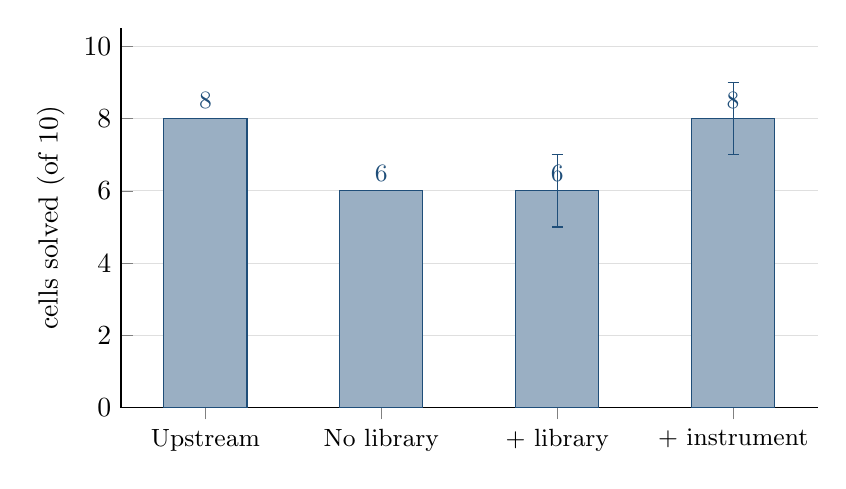
\begin{tikzpicture}
\begin{axis}[
    width=0.86\textwidth, height=6.4cm,
    ybar, bar width=30pt,
    ymin=0, ymax=10.5, ytick={0,2,4,6,8,10},
    ylabel={cells solved (of 10)},
    symbolic x coords={Upstream, {No library}, {+ library}, {+ instrument}},
    xtick=data,
    x tick label style={font=\small, align=center},
    nodes near coords, nodes near coords style={font=\small\bfseries, color=acc},
    enlarge x limits=0.16,
    ymajorgrids, grid style={gray!25},
    axis lines*=left,
]
\addplot[fill=acc!45, draw=acc, error bars/.cd, y dir=both, y explicit,
         error bar style={acc}]
  coordinates {
    (Upstream,8)        +- (0,0)
    ({No library},6)    +- (0,0)
    ({+ library},6)     +- (0,1)
    ({+ instrument},8)  +- (0,1)
  };
\end{axis}
\end{tikzpicture}
\caption{Cells solved per arm. Upstream is a single sweep with answer files
available; the three clean-room arms are means of three passes with answer files
unreachable. Bars show the spread across passes.}
\end{figure}

\noindent
The library arms are worth stating plainly because the result is negative:
\textbf{no library tier produces a measurable suite-wide lift}. No library,
promoted memory, and blind task playbooks are indistinguishable at 6.0. An
earlier reading of these same experiments claimed $+0.7$ cells for the memory
library; that figure was an artefact of a harness crash in one early sweep, and
when a fresh no-library sweep was run at current code it scored 6, giving the
no-library arm $6,6,6$ with zero spread. The claim is retired.

What the library \emph{does} buy is cell-targeted and invisible in a mean: task
t6 went from 0/11 across the clean-room era and 0/3 in the no-library arm to
\textbf{5/6} once four gated playbook entries existed (Section~4).

\subsection{The controlled ablation}

Blind library arm versus the same arm with the instrument armed: same sandbox,
same library, same model, same turn budget, same ten cells, three passes each.
\vt{} is the only variable. Nothing else in this project is this clean.

\begin{table}[htbp]
\centering
\small
\begin{tabular}{@{}l c c c l@{}}
\toprule
\textbf{Cell} & \textbf{Blind} & \textbf{Instrument} & \textbf{$\Delta$} & \textbf{Reading} \\
\midrule
t0 & 0/3 & \textbf{3/3} & \textbf{+3} & unpredicted; carries the result \\
t1 & 3/3 & 2/3 & $-1$ & noise \\
t2 & 3/3 & 3/3 & 0 & saturated \\
t3 & 2/3 & 3/3 & $+1$ & noise \\
t4 & 2/3 & 3/3 & $+1$ & noise \\
t5 & 0/3 & 1/3 & $+1$ & the designed target --- moved weakly \\
t6 & 2/3 & 2/3 & 0 & knowledge-bound; predicted indifferent \\
t7 & 3/3 & 3/3 & 0 & saturated \\
t8 & 0/3 & \textbf{3/3} & \textbf{+3} & unpredicted; carries the result \\
t9 & 3/3 & \textbf{1/3} & \textbf{$-2$} & regression, unexplained \\
\midrule
\textbf{Suite} & \textbf{6.0} & \textbf{8.0} & \textbf{+2.0} & \\
\bottomrule
\end{tabular}
\caption{The single-variable ablation. The entire suite gain is t0 and t8; every
other cell nets to zero.}
\end{table}

\noindent
\textbf{The gain is two cells, not a general uplift.} That is a sharper and less
flattering statement than the mean, and it is the one the data supports. In the
records, the instrument is used early and for object identity discrimination in
all six t0/t8 runs --- its designed role --- but some of its answers in those
very runs are wrong, and no matched-pair counterfactual exists. \textbf{No
causal claim is made for t0 and t8.} They are the next diagnostic target.

\subsection{Generation state}

The library is grown in generations: clean start, sweep, mine observations,
human review, apply, next sweep. The table below carries the current state and
is designed to take one more row when the next generation completes.

\begin{table}[htbp]
\centering
\small
\begin{tabularx}{\textwidth}{@{}l l c X@{}}
\toprule
\textbf{Generation} & \textbf{Arm} & \textbf{Suite} & \textbf{What changed} \\
\midrule
Gen 0--5 & clean-room + library & 6.0 & five gate cycles; no suite-wide lift \\
Gen 5 + playbooks & blind practice & 6.0 & task-tier entries; t6 cracked \\
\rowcolor{soft} Gen 6 & practice + instrument & \textbf{8.0\,$\pm$\,1.0} &
  vision channel added as a tool \\
\rowcolor{soft} Gen 7 & practice + instrument, repaired library & \textbf{8.67\,$\pm$\,0.58} &
  issue 5f closed; t9 resident mined in; \textbf{t5 0/3$\rightarrow$3/3}, \textbf{t9 1/3$\rightarrow$3/3}, \textbf{t1 3/3$\rightarrow$0/3} \\
\bottomrule
\end{tabularx}
\caption{Generation state. Each row is a fingerprinted configuration, not a
narrative stage.}
\end{table}

% ================================================================
\section{Case study: t6, a knowledge wall}

t6 is the cell that justifies the memory machinery. Under the clean-room
sandbox it failed eleven consecutive times, and the no-library arm still fails
it 0/3. It is now solved 5 times in 6 attempts. The mechanism is worth following
because every step is on disk.

\textbf{The control arm ran first.} An amnesiac between-episode loop --- attempt,
observe, update the playbook, attempt again --- ran five rounds over 115
minutes and self-terminated with the literal string \texttt{"no new knowledge"}:
zero solves, two entries admitted. Its last two rounds used the same playbook
the experimental arm would start from, which is what makes the comparison
knowledge-fair.

\textbf{What the resident session found} was a contrast that a fresh-context
loop structurally cannot form, because it requires holding two attempts in one
context. The same grasp prompt, on the same cell, before and after a single
pre-positioning move:

\begin{evidence}[title={The discriminator, from \texttt{attempt\_01/tool\_calls.jsonl}}]
\ttfamily\footnotesize
seq 41 --- pi0\_pick("pick up the flat butter slab")\\
\hspace*{2em}success: \textbf{true}\quad min\_gripper\_opening: \textbf{0.0020}\\[0.4em]
seq 50 --- pi0\_pick("pick up the flat butter slab")\ \ \textrm{\emph{(after one pre-position)}}\\
\hspace*{2em}success: \textbf{true}\quad min\_gripper\_opening: \textbf{0.0394}
\end{evidence}

\noindent
The slab is 40\,mm. The first pick closed to 2\,mm --- on air --- and reported
success. The harness's own geometry caught it at the next call, and the wording
of that tool result is the reason the agent believed the measurement over the
flag: \emph{``the points below the eef are geometry, not a grasped object
\ldots\ gripper width alone cannot tell these apart --- it read the same on
steps that were holding and steps that were not.''}

\textbf{The model wrote its own diagnosis} into the reset call, which is schema-%
required to state a change rather than permit a rerun:

\begin{evidence}[title={The model's reset reason, verbatim (live log, seq 1)}]
\small\itshape
``Attempt 1 SOLVED \ldots\ (2) pre-position at (0.05,\,-0.101,\,0.15) gripper open
then \texttt{pi0\_pick}(`pick up the flat butter slab') --- real grasp shows final finger
opening 0.039 (pinching the 0.04 slab) vs air grasp 0.002 \ldots\ \textbf{first
pick from home air-grasped, so pre-positioning above the butter is the decisive
rung.}''
\end{evidence}

\noindent
Two proposals were mined from that session. Both were \emph{held} by the gate's
contract check --- revising an existing entry requires human confirmation ---
and both were approved by a human before entering the library. The subsequent
seed-0 exams, single attempt and with no resident tooling on the surface, solved
3/3 at environment steps 8, 15 and 7, with a fourth solve in the next full
sweep. Cross-seed transfer was \textbf{2/3}: two seeds solved, one failed.

\begin{caution}[title={A claim this project had to correct about itself}]
This result was written down internally as ``t6: 0/11 all-time''. That is false.
t6 seed 0 was solved 6/7 times \emph{before} the sandbox existed, and 4 of those
runs read \cit{results\_object\_pert/object\_swap\_t6\_s0.json} --- the answer
for that exact cell. The accurate claim is \textbf{0/11 in the clean-room era},
and it is the stronger one: removing the answer killed the cell for eleven runs,
and the harness re-derived a working recipe by measurement.
\end{caution}

% ================================================================
\section{Case study: t5, a perception wall and a mechanism misfire}

t5 requires distinguishing two visually similar sauce containers. Its wall is
not knowledge and not policy: the discriminating attribute has no measuring
channel. A blind resident session on this cell ended in a way worth quoting,
because it is what running out of measurable options looks like from inside:

\begin{evidence}[title={Blind session, model output at turn 16, then turns 18--19}]
\small
\emph{``Wrist probes on A are all within noise (tomato 0.551, bbq 0.574, red
0.637, brown 0.602) --- language cannot separate the two sauce bottles.''}

\medskip
\ttfamily\footnotesize
turn 17\quad out=35{,}814\qquad turn 18\quad out=44{,}006\qquad turn 19\quad out=52{,}198
\end{evidence}

\noindent
Turns 18 and 19 emitted no text and no tool call, and each consumed exactly
8{,}192 output tokens --- the entire generation budget, spent inside the hidden
reasoning channel. The run died at turn 19 of 150. It did not fail at the task;
it tried to settle a perceptual question by thinking.

\subsection{The instrument, and both of its faces}

The vision channel enters as a \emph{tool}, not a planner swap: one call sends
one on-disk image to a cheap VLM and returns the reply verbatim, with the exact
text sent recorded alongside it. The reader is given no task context, so it
cannot smuggle a task decision past the planner, and the tool exists only when
the run is armed --- a blind arm does not ship a tool it cannot honour.

Within a single session the channel both rescued and misled. A pixel answer
back-projected to $z=0.029$\,m --- table level, usable --- and the re-pick
succeeded. A different pixel answer back-projected to $z=0.132$\,m, the height
of a milk carton, and when the same view was re-cropped and re-asked the reader
replied: \emph{``The object in the center is the milk carton; no small red
tomato sauce bottle is visible.''} That pair is why the admitted rule is a
height sanity check rather than a prohibition.

\subsection{The failures, adjudicated}

Under the instrument t5 moved only 0/3 to 1/3. The two failures were adjudicated
by a procedure fixed \emph{before} the sweep produced any number, and the answer
is not the one the design anticipated. \textbf{The instrument was right and the
planner overruled it.}

Ground truth, from the solved run: the target is a silver \emph{can} with a
red/green label; the brown \emph{bottle} at $[-0.19,\,-0.07]$ reads ``TANGY BBQ
SAUCE''. Both failures picked the bottle, after the reader had correctly said
so, on this inference --- quoted from the agent's own audit:

\begin{evidence}[title={The failing inference, verbatim}]
\small\itshape
``since the env guarantees a pickable \texttt{tomato\_sauce\_1} and exactly one bottle
exists on the table, the standing bottle was taken as the tomato sauce.''
\end{evidence}

\noindent
The tomato sauce is a can. ``The only bottle'' is the distractor by
construction.

\subsection{The most important negative result: a gated entry became an excuse}

Both failures then explained their non-firing termination flag by citing an
entry from our own promoted library --- an env-tier entry, read by every cell,
whose closing clause reads: \emph{``If the object is confirmed inside the basket
and the origin is empty but termination has not fired, treat the task as
complete; do not keep re-seating the object.''}

The checker was right: a BBQ bottle was in the basket. The entry handed a
wrong-object run a ready-made, honest-sounding reason to stop looking.

\begin{caution}[title={Why no gate check could have caught this}]
The entry is true. Its citations resolve, its numbers trace to the records they
cite, and its own \texttt{counter\_evidence} block honestly declares a case where
its recipe failed. It was admitted correctly. The defect is that its stopping
condition keys on the \emph{observation} ``the flag did not fire'' without
discriminating \emph{why} --- so it fires identically when the checker is wrong
and when the checker is right. Across the instrument arm, \textbf{four of six
failures ended with the agent believing it had succeeded}, and three cited this
licence explicitly. It is grown knowledge that licenses giving up.
\end{caution}

\noindent
This also revises a claim made earlier in the project's own notes: of three
recorded cases where the flag failed to fire on this cell, two are now explained
by the wrong object being placed. The flaky-checker evidence is thinner than
previously written.

% ================================================================
\section{What the upstream score is made of}

The comparison a reviewer will ask for is what the harness we replaced scores.
Upstream main, cloned standalone, same model, same turn budget, its own prompt,
its priors sync left enabled: \textbf{8/10} in 45 minutes.

That score is purchased, and the receipt is legible in one cell. t5 --- the cell
that cost us a resident session, an instrument and three adjudicated library
entries --- upstream solved at environment step 2:

\begin{evidence}[title={Upstream t5, the entire run}]
\ttfamily\footnotesize
reads:\ \ results\_object\_pert/object\_swap\_t5\_s0.json\ \ \ \ x3\\
\hspace*{3.4em}results\_object\_pert/recipe\_object\_swap\_t5\_s0.jsonl\ \ x2\\[0.4em]
step 1\ \ pi0\_pick("pick up the tomato sauce")\\
step 2\ \ pi0\_pick("pick up the tomato sauce")\ \ $\rightarrow$\ \ terminated
\end{evidence}

\noindent
No segmentation, no localisation, no perception of any kind: two identical
policy calls replayed off the stored solution. This is not a criticism of
upstream --- with the answers on disk it is the rational move, and the priors
are part of that design. It is the reason the number cannot be read as a
measurement \emph{of a harness}. Removing the answer files costs two cells;
winning them back has to be done by a mechanism.

% ================================================================
\section{Predictions, filed before the numbers existed}

Before the instrument sweep ran, per-cell predictions were recorded and
timestamped so that the result could not be narrated afterwards. They were
substantially wrong, in an informative direction.

\begin{table}[htbp]
\centering
\small
\begin{tabularx}{\textwidth}{@{}X l@{}}
\toprule
\textbf{Prediction (filed before any run)} & \textbf{Outcome} \\
\midrule
t5 should move; it is the designed target & \textbf{partly wrong} --- 0/3 to 1/3, and its failures were not vision failures \\
t6 unchanged; its wall is knowledge & \textbf{correct} --- 2/3 to 2/3 \\
t1, t2, t7, t9 saturated and unchanged & \textbf{wrong for t9} (3/3 to 1/3); correct otherwise \\
t3, t4 noise-dominated, $\pm 1$ & correct \\
t0, t8: prediction explicitly declined & 0/3 to \textbf{3/3} each --- and they are the entire gain \\
\bottomrule
\end{tabularx}
\caption{The pre-registration scorecard.}
\end{table}

\noindent
The mechanism model was wrong about \emph{where} the instrument's value would
appear. It was built for t5 and predicted irrelevant elsewhere; it barely moved
t5 and carried two cells instead. Declining to predict t0 and t8 was the correct
call, and the reason they were unpredictable is that nobody had ever diagnosed
why they failed.

One filed commitment has to be applied to its author. The pre-registration said
the single number to distrust on sight would be a large suite jump without t5
moving --- which is exactly what happened. The rule does not fire, because the
movement is concentrated in two chronic zeros at $+3$ each, which noise at $n=3$
cannot manufacture. It is recorded here rather than quietly dropped.

% ================================================================
\section{Negative results, limits, and retired claims}

\textbf{Retired: the generational growth curve.} Single-run scores across five
library generations read $4 \to 5 \to 7 \to 6 \to 5$ and looked like growth. Under
repeats the curve vanished.

\textbf{Retired: the ``+0.7 cells'' library effect.} It was an artefact of a
DeepSeek request-integrity crash in one early sweep, fixed since. A fresh
no-library sweep at current code scored 6, giving $6,6,6$ with zero spread.

\textbf{Unexplained: the t9 regression.} t9 went 3/3 to 1/3 under the
instrument. The pre-registered explanation --- turns burned on instrument calls
--- is refuted by the records: one of the two failures called the instrument
\emph{zero} times, and both used exactly 46 tool calls. Both picked the correct
object with real grasps and stopped on the stopping licence described in
Section~5.3.

\textbf{Arming is not using.} Three of the thirty instrument-arm runs carried
the flag and never called the tool. They are functionally blind runs in the
instrument column, which makes the $+2.0$ a mild understatement of what
\emph{using} the instrument is worth and an overstatement of what \emph{arming}
it is worth.

\textbf{Sample sizes.} Every clean-room arm is $n=3$ passes of ten cells. The
upstream arm is $n=1$. Cross-seed transfer on t6 is $n=3$, of which one failed.
t5's solved exam on the scoring seed is $n=1$.

\textbf{Generation 7 gained two cells and lost one.} Repairing the library took
t5 from 1/3 to \textbf{3/3} and t9 from 1/3 to \textbf{3/3}, and the suite mean
to 8.67\,$\pm$\,0.58 --- while t1 fell to 0/3. The entry revision is not the
cause: two of the three t1 failures never read the revised entry, all three died
on \texttt{reached max\_turns} rather than stopping early, and a licence-assisted
solve is impossible to lose because it was never a counted solve (the flag stays
silent, so it already scored as a failure). The measured cause is a perception
spiral --- motion calls flat at 9--12 while perception calls climb 32 to 153 ---
i.e.\ a known failure mode returning with the instrument as a new channel to
spiral in. Remedy filed, not built; $n=3$.

\textbf{No frontier comparison exists.} The only baseline is the same model on
the upstream harness. No head-to-head against a stronger model has ever been
run, and none is claimed.

\textbf{Not shipped.} A code-as-policy arm was implemented faithfully to a
published algorithm, produced no measured result, and is excluded from the
reviewed branch rather than presented as a capability.

% ================================================================
\section{Reproduction}

Every claim above is recomputable from the run archive without the agent
framework installed. Scores come from \texttt{states.json}; the per-call record
including read-only calls comes from \texttt{tool\_calls.jsonl}; each run's
boundary comes from its \texttt{sandbox.json} fingerprint.

\begin{evidence}[title={Checks}]
\ttfamily\footnotesize
\# did a run consume a prior?  (empty for every sandboxed run)\\
grep 'read\_text\_file' run.log | grep -E 'results\_.*\_pert|env\_calibration'\\[0.5em]
\# rebuild any run's evidence from disk alone\\
python -m rpent.replay \textless run\_dir\textgreater\\[0.5em]
\# the regression suite: no API key, no GPU\\
for t in deep\_agent resident vision\_tool tool\_docs prompt\_leveling sandbox \textbackslash\\
\hspace*{2.2em}databus shape gate practice replay; do python tests/harness/test\_\$t.py; done
\end{evidence}

\noindent
Replay rebuilds a finished run as a turn-by-turn timeline from the disk
artifacts alone, and reports its own incompleteness under a heading of
\emph{record gaps}. That constraint is deliberate: a gap means the logs are
missing something, and the remedy is to record more, not to improve the
renderer.

\end{document}
